\section{Analysis of the drone} \label{sec:droneSpec}
For this project a 3DR Solo drone is made available. In order to make system requirements it is needed to know some parameters and specifications of the 3DR Sole drone. 

Table \ref{tab:DroneSpecs} shows the specifications of the 3DR Sole drone. 
\begin{table}[h]
	\centering
	\caption{The parameters and specifications of the 3DR Solo drone.} \label{tab:DroneSpecs}

	\begin{tabularx}{\textwidth}{lX}
		Specification 		&  								\\ \toprule \rowcolor{lightGrey}
		Maximum Speed		&  \SI{55}{\mph} (\SI{89}{\kilo\meter\per\hour} $\approx$ \SI{24.722}{\m\per\second})								\\
		Fly time 			& \SI{20}{\minute}; \SI{15}{\minute} with payload (may vary)	\\ \rowcolor{lightGrey}
		Range 		 		& \SI{0.6}{\miles} (\SI{1}{\kilo\meter})									\\
		Max payload			& \SI{0.8}{\kilogram} 											\\ \rowcolor{lightGrey}
		Max altitude		& \SI{400}{\feet} per FAA regulation, user adjustable (\SI{122}{\meter})\\
		Motors				& \SI{880}{\kilo\volt} 											\\ \rowcolor{lightGrey}
		Communication		& 3DR Link secure WiFi network 						\\
		Frequency			& \SI{2.4}{\giga\hertz} 											\\ \rowcolor{lightGrey}
		Dimensions			& \SI{10}{\inch} tall (\SI{25}{\centi\meter}), \SI{18}{\inch} (\SI{46}{\centi\meter}) motor-to-motor\\
		Flight battery		& Lithium polymer \SI{5200}{\milli\ampere\hour}, \SI{14.8}{\volt} in DC 				\\ \rowcolor{lightGrey}
		Battery charge time	& \SI{1.5}{\hour} (may vary)								\\
		Max ascent speed	& \SI{10}{\meter\per\second} in Stabilized mode; \SI{5}{\meter\per\second} in FLY mode		\\ 
	\end{tabularx}
	\caption*{\citep{Web:DroneSpec}}
\end{table}

\subsection{Required precision} \label{sec:RequiredPrecision}
As of \autoref{ch:ProblemStatement} a laser pointer is made available for this project. It is chosen that the goal is to hit the drone with it. 

In this subsection the required precision to hit the drone with the laser pointer is determined. This requirement is the criterion to evaluate the feasibility of the different tracking methods in the later part of this chapter. 
 
The trigonometric model on \autoref{fig:RequiredPrecision} is made to calculate the required precision when the beam is pointing at the center of the drone. 
\begin{figure}[h!]
    \centering
        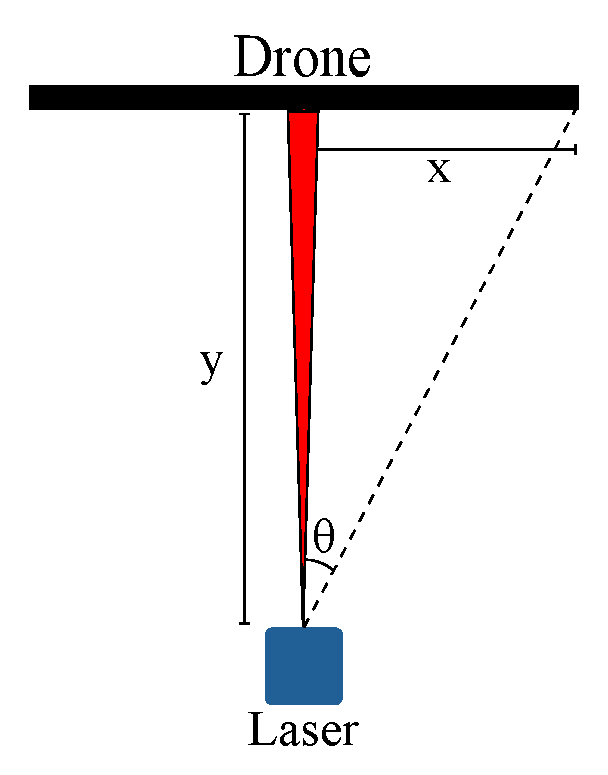
\includegraphics[width=0.4\textwidth]{figures/tracking/required_precision.pdf}
        \caption{Illustration of the laser pointing at the drone. $\theta$ is the maximum angular deviation the tracking module can have while still hitting the target.}
        \label{fig:RequiredPrecision}
\end{figure}

\newpage
From \autoref{fig:RequiredPrecision} \autoref{eq:GeneralRequiredPrecision} is derived. 
\begin{equation} \label{eq:GeneralRequiredPrecision}
\theta = \arctan \left( \frac{x}{y} \right) \addunit{\radian}
\end{equation}
\startexplain
\explain{$\theta$ is the angular precision}{\si{\radian}}
\explain{$x$ is half the size of the drone}{\si{\meter}}
\explain{$y$ is the distance from the laser to the drone}{\si{\meter}}
\stopexplain
Because the laser is purely for demonstration purposes, beam spreading is not taken into account. 

In order to calculate the required precision a choice of the maximum operation range of the drone is needed. Since the system is a charging station for a drone it is assumed that the drone is able to move to the charging station. Since this is a proof of concept, it is chosen that a maximum operation range of \SI{120}{\meter} is sufficient. \SI{120}{\meter} is chosen because it is approximately the maximum altitude of the 3DR Solo drone. 

With the maximum operation distance of \SI{120}{\meter} and a drone size of approximately \SI{500}{\milli\meter}, \autoref{eq:GeneralRequiredPrecision} can be used to calculate the required precision, as seen in \autoref{eq:RequiredPrecision}. 
\begin{equation}\label{eq:RequiredPrecision}
\theta_{\SI{120}{\meter}} = \arctan \left( \frac{{\dfrac{\SI{500}{\milli\meter}}{2}}}{\SI{120}{\meter}} \right) \approxeq \SI{2,083}{\milli\radian} 
\end{equation}
 

Now the required precision is found to be \SI{2.083}{\milli\radian} and the needed angular velocity is researched.

\subsection{Required angular velocity of the motor stand}\label{sec:NeedForSpeed}
In this section the required angular velocity of the motorised antenna stands rotation is found. This speed is needed in order to do system requirements in \autoref{ch:SystemRequirements}.
\begin{equation} \label{eq:NFS3} 
\omega = \frac{2\pi}{t} = \frac{2\pi}{\frac{C}{v}} = \frac{2\pi}{\frac{2\pi \cdot r}{v}} \addunit{\radian \per \second}
\end{equation}
\startexplain
\explain{$\omega$ is the minimum speed}{\si{\radian \per \second}}
\explain{$t$ is the round time or circulation time}{\si{\meter}}
\explain{$C$ is the circumference}{\si{\meter}}
\explain{$v$ is the speed of the drone}{\si{\meter \per \second}}
\explain{$r$ is the distance to the drone}{\si{\meter}}
\stopexplain

In section \autoref{sec:RequiredPrecision} it is chosen that the prototype should work at ranges up to \SI{120}{\meter} in order to calculate the required precision. In order to determine the required angular velocity of the motor stand a minimum operation range have to be defined as well. Since the drone is not completely steady in the air, some guard distance between the antenna stand and the drone is desired. The minimum operation range is chosen to \SI{20}{\meter}, this is arbitrarily decided based on the estimated needed safety distance and for an approximation needed by some tracking methods seen later in the chapter.  


Inserting the the minimum operation range and the speed of the drone (found in \autoref{sec:droneSpec}) into \autoref{eq:NFS3}, yield the needed angular velocity of the motor stand, as seen in \autoref{eq:NFS4}. 
\begin{equation} \label{eq:NFS4} 
\omega = \frac{2\pi}{\frac{2\pi \cdot 20}{24.722}} = \SI{1.2361}{\radian \per \second}
\end{equation}